%This is a template file for use of iopjournal.cls

\documentclass{iopjournal}
\bibliographystyle{IEEEtran}
\usepackage{float}
\usepackage{amsmath}
\usepackage{tikz}

% Options
%  [anonymous]  Provides output without author names, affiliations or acknowledgments to facilitate double-anonymous peer-review
%
% The following packages are required by iopjournal.cls and do not need to be declared again:
%  graphicx
%  fancyhdr
%  xcolor
%  hyperref
%

\begin{document}

\articletype{Tarea 3} %	 e.g. Paper, Letter, Topical Review...

\title{Descenso de Gradiente}

\author{Daniel González$^1$\orcid{0000-0000-0000-0000}}

\affil{$^1$Facultad de Ingeniería, Universidad Autónoma de Querétaro, Querétaro, México \\ 21/08/2025}

\email{dgonzalez16@alumnos.uaq.mx}

\keywords{descenso gradiente, plano, mínimo, derivada, epocas}

\begin{abstract}
El descenso de gradiente consiste en tomar el principio de la gradiente la cual nos indica en tomar la ruta del punto más alto de una función, sin embargo en este caso al tomar la dirección contraria encontraríamos el punto más bajo. Imaginemos que estamos en una montaña, y quisiéramos encontrar el punto más bajo con esto podríamos avanzar paso a paso en la dirección de mayor pendiente descendente hasta llegar al mínimo.
\end{abstract}

\section{Introducción}

El descenso de gradiente es un método iterativo para encontrar el mínimo de una función.  
Dada una función
\[
f(\theta),
\]
donde $\theta$ representa los parámetros, el objetivo es encontrar el valor de $\theta$ que minimiza $f$.

\begin{itemize}
    \item El gradiente es el vector de derivadas parciales:
    \begin{equation}
    \nabla f(\theta) = \left( \frac{\partial f}{\partial \theta_1}, \frac{\partial f}{\partial \theta_2}, \dots, \frac{\partial f}{\partial \theta_n} \right).
    \label{d_parcial}
    \end{equation}


    \item La actualización de parámetros se realiza con la regla:
    \[
    \theta \leftarrow \theta - \eta \, \nabla f(\theta),
    \]
    donde $\eta > 0$ es la tasa de aprendizaje.
\end{itemize}

Al repetir este proceso varias veces, los parámetros $\theta$ se acercan a un mínimo de la función.


En machine learning, la función $f(\theta)$ corresponde a la función de pérdida o error, que mide qué tan bien predice el modelo.  
El descenso de gradiente ajusta los parámetros (por ejemplo, los \emph{pesos} de una red neuronal) para minimizar dicho error y así mejorar el desempeño del modelo.

\subsubsection*{Ejemplo gráfico}

\begin{center}
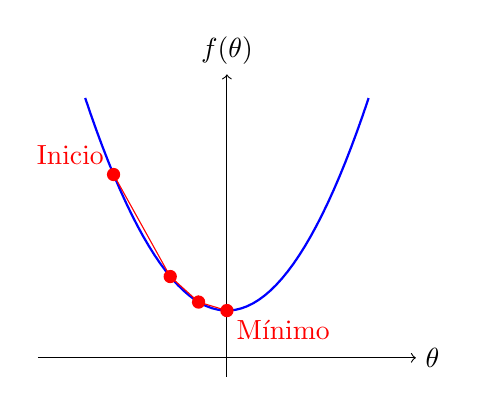
\begin{tikzpicture}[scale=1.2]
  % Ejes
  \draw[->] (-2,0) -- (2,0) node[right] {$\theta$};
  \draw[->] (0,-0.2) -- (0,3) node[above] {$f(\theta)$};
  
  % Curva cuadrática
  \draw[thick, blue, domain=-1.5:1.5, samples=50] plot (\x,{(\x)^2+0.5});
  
  % Puntos de iteraciones
  \fill[red] (-1.2,1.94) circle (2pt) node[above left] {Inicio};
  \fill[red] (-0.6,0.86) circle (2pt);
  \fill[red] (-0.3,0.59) circle (2pt);
  \fill[red] (0,0.5) circle (2pt) node[below right] {Mínimo};
  
  % Flechas
  \draw[->, red] (-1.2,1.94) -- (-0.6,0.86);
  \draw[->, red] (-0.6,0.86) -- (-0.3,0.59);
  \draw[->, red] (-0.3,0.59) -- (0,0.5);
\end{tikzpicture}
\end{center}

\section{Desarrollo}
Se plantea la función inicial:
\begin{equation} \label{ec_init}
\begin{aligned}
   z &= x^3 + x^2 + y^3 + y^2 \\
   z &= \theta_0^3 + \theta_0^2 + \theta_1^3 + \theta_1^2
\end{aligned}
\end{equation}

Partiendo de la ecuación ~\ref{d_parcial} calculamos la derivada parcial de esta para obtener:

\begin{equation}
    \frac{\partial}{\partial x} = 3x^2 + 2x
\end{equation}
\begin{equation}
    \frac{\partial}{\partial y} = 3y^2 + 2y
\end{equation}

Una vez que tenemos esto, ya podemos obtener nuestra función para calcular el descenso de gradiente.
El \textbf{gradiente} de $z$ es:
\begin{equation}
\nabla z(\boldsymbol{\theta}) =
\begin{bmatrix}
\frac{\partial z}{\partial \theta_0} \\
\frac{\partial z}{\partial \theta_1}
\end{bmatrix}
=
\begin{bmatrix}
3\theta_0^2 + 2\theta_0 \\
3\theta_1^2 + 2\theta_1
\end{bmatrix}.
\label{eq:grad}
\end{equation}

Con un \textit{learning rate} $\eta>0$, la regla de actualización iterativa (descenso de gradiente) es:
\begin{equation}
\boldsymbol{\theta}^{(k+1)} \;=\; \boldsymbol{\theta}^{(k)} \;-\; \eta \,\nabla z\!\left(\boldsymbol{\theta}^{(k)}\right),
\label{eq:gd_update}
\end{equation}
es decir, componente a componente:
\begin{align}
\theta_0^{(k+1)} &= \theta_0^{(k)} - \eta\,\big(3(\theta_0^{(k)})^2 + 2\theta_0^{(k)}\big), \\
\theta_1^{(k+1)} &= \theta_1^{(k)} - \eta\,\big(3(\theta_1^{(k)})^2 + 2\theta_1^{(k)}\big).
\end{align}

Con esto en mente pasamos al código para poder evaluar el plano de nuestra función, con nuestras $\theta_0$ y $\theta_1$ iniciales así como un learning rate que sera $\alpha$ y un numero de épocas.

Nuestros valores serán:
\begin{equation}\label{condiciones_iniciales}
    \begin{aligned}
        \theta_0 = 0.5 \\
        \theta_1 = 0.5 \\
        \alpha = 0.01 \\
        epoch = 5000
    \end{aligned}
\end{equation}

Con estos valores vamos a mostrar las iteraciones en nuestra gráfica y obtenemos lo siguiente:
\begin{figure}[H]
 \centering
        \includegraphics[width=0.5\textwidth]{rsc/gradiente_descendiente.png}
 \caption{Grafica del plano de la ecuacion\ref{ec_init} con gradiente descendente apartir de las condiciones \ref{condiciones_iniciales}}
\label{fig1}
\end{figure}

Como se puede ver nuestro gradiente tiende a cero.

\section{Conclusiones}
El descenso de gradiente confirma encontrar mínimos en funciones de varias variables.  
A partir de la función propuesta y del cálculo de sus derivadas parciales, se pudo construir la regla de actualización que, con ayuda de un ciclo de iteraciones, nos guía hacia valores donde el gradiente tiende a cero como se ve en la figura \ref{fig1}.  

Durante el desarrollo podemos ver cómo la elección de una tasa de aprendizaje adecuada y un número suficiente de épocas permiten visualizar la convergencia de los parámetros al mínimo local de la función. También se destacó la relevancia de este procedimiento en machine learning, donde el descenso de gradiente se utiliza para ajustar los parámetros de un modelo y minimizar la función de pérdida, mejorando así su capacidad predictiva.  

Con esto es posible demostramos la base matemática así como la aplicación práctica del descenso de gradiente, la cual es una herramienta fundamental en optimización y aprendizaje automático.


%\begin{thebibliography}{00}
%\bibliography{references}
%\end{thebibliography}


\end{document}


